%==============================================================================
% Sjabloon onderzoeksvoorstel bachelorproef
%==============================================================================%
% Compileren in TeXstudio:
%
% - Zorg dat Biber de bibliografie compileert (en niet Biblatex)
%   Options > Configure > Build > Default Bibliography Tool: "txs:///biber"
% - F5 om te compileren en het resultaat te bekijken.
% - Als de bibliografie niet zichtbaar is, probeer dan F5 - F8 - F5
%   Met F8 compileer je de bibliografie apart.
%
% Als je JabRef gebruikt voor het bijhouden van de bibliografie, zorg dan
% dat je in ``biblatex''-modus opslaat: File > Switch to BibLaTeX mode.

\documentclass{hogent-article}

\usepackage{lipsum} % Voor vultekst

\usepackage[dutch]{babel}
\usepackage[utf8]{inputenc}
\usepackage{hyperref}

\usepackage[backend=biber,style=apa]{biblatex}
\DeclareLanguageMapping{dutch}{dutch-apa}
\addbibresource{bibliografie.bib}

%------------------------------------------------------------------------------
% Metadata over het artikel
%------------------------------------------------------------------------------

%---------- Titel & auteur ----------------------------------------------------

% TODO: (fase 2) geef werktitel van je eigen voorstel op
\PaperTitle{een onderzoek over gamificatie in het leren van een vreemde taal: welke spelelementen kunnen specifiek worden
    gebruikt om leerresultaat in LFL te verbeteren}
% Dit is typisch de opdracht en het vak waarvoor dit artikel geschreven is, bv.
% ``Verslag onderzoeksproject Onderzoekstechnieken 2018-2019''
\PaperType{Paper Research Methods: onderzoeksvoorstel}

% TODO: (fase 1) vul je eigen naam in als auteur, geef ook je emailadres mee!
\Authors{Arne Verbanck\textsuperscript{1}, Gustavo Van Eenooghe\textsuperscript{2}} % Authors

% Als het hier effectief gaat om een voorstel voor de bachelorproef, dan ben je
% hier verplicht de naam van je co-promotor in te vullen. Zoniet, dan kan je het
% leeg laten.
\CoPromotor{}

% Contactinfo: Geef hier de contactgegevens van elke auteur van het artikel (en
% indien van toepassing ook van de co-promotor).
\affiliation{
  \textsuperscript{1} \href{mailto:ArneVerbanck@student.hogent.be}{ArneVerbanck@student.hogent.be}}
\affiliation{
  \textsuperscript{2} \href{mailto:GustavoVanEenooghe@student.hogent.be}{GustavoVanEenooghe@student.hogent.be}
}

%---------- Abstract ----------------------------------------------------------

\Abstract{% TODO: (fase 6)
Hier schrijf je de samenvatting van je artikel, als een doorlopende tekst van één paragraaf.

Bij de sleutelwoorden geef je het onderzoeksdomein (= specialisatierichting in de opleiding), samen met andere sleutelwoorden die je werk beschrijven.
}

%---------- Onderzoeksdomein en sleutelwoorden --------------------------------
% TODO: (fase 2) Vul de sleutelwoorden aan.

% Het eerste sleutelwoord beschrijft het onderzoeksdomein. Je kan kiezen uit
% deze lijst:
%
% - Mobiele applicatieontwikkeling
% - Webapplicatieontwikkeling
% - Applicatieontwikkeling (andere)
% - Systeembeheer
% - Netwerkbeheer
% - Mainframe
% - E-business
% - Databanken en big data
% - Machineleertechnieken en kunstmatige intelligentie
% - Andere (specifieer)
%
% De andere sleutelwoorden zijn vrij te kiezen.

\Keywords{Onderzoeksdomein; Applicatieontwikkeling; Andere(Gamificatie);}
\newcommand{\keywordname}{Sleutelwoorden} % Defines the keywords heading name

%---------- Titel, inhoud -----------------------------------------------------

\begin{document}

\flushbottom % Makes all text pages the same height
\maketitle % Print the title and abstract box
\tableofcontents % Print the contents section
\thispagestyle{empty} % Removes page numbering from the first page

%------------------------------------------------------------------------------
% Hoofdtekst
%------------------------------------------------------------------------------

\section{Inleiding}

% TODO: (fase 2) introduceer je gekozen onderwerp, formuleer de onderzoeksvraag en deelvragen. Wat is de doelstelling (is die S.M.A.R.T.?), wat zal het resultaat zijn van het onderzoek (een Proof-of-Concept, een prototype, een advies, ...)? Waarom is het nuttig om dit onderwerp te onderzoeken?



Met het opkomen van de ‘digitale autochtonen’ of digital natives zijn studenten veranderd. De leraren en onderwijsstrategieën moeten zich aanpassen aan deze nieuwe groep leerlingen om de noodzakelijke samenhang te creëren en het maximale potentieel uit hen te halen. Door de mobile telefoon en sociale media zit men met kortere aandacht spanne en over het algemeen hogere fluctuaties van het dopamine niveau. Als antwoord hierop is de interesse in ‘gamificatie’, oftewel game elementen implementeren in het dagelijkse leven, enorm toegenomen in het afgelopen decennia. In dit onderzoek proberen we uit de weid verspreide literatuur een consensus te scheppen. We gaan systematisch game elementen in de educatieve sector, specifiek bij het leren van een nieuwe taal, bekijken en waarom ze werken.
\section{Overzicht literatuur}

% TODO: (fase 4) schrijf de literatuurstudie uit en gebruik waar gepast referenties naar de vakliteratuur.

% Refereren naar de literatuur kan met:
% \autocite{BIBTEXKEY} -> (Auteur, jaartal)
% \textcite{BIBTEXKEY} -> Auteur (jaartal)
Lacunes in de beschikbare middelen
Hoewel er over dopamine heel veel te zeggen valt en er verscheidene soorten dopamine en dopaminereceptoren zijn gaan we hier niet dieper op in. Hetzelfde geld voor de andere drie hormonen die we aanhalen in dit onderzoek waar nog minder over geweten is. Dit doen we omdat dit niet de focus is van het onderzoek en we onszelf niet vaardig genoeg in het onderwerp achten om dit op een representatieve manier over te brengen.
Probleemstelling
Hoewel er veel documentatie over spellen en hoe ze gemaakt zijn bestaat zijn weinig kwalitatieve onderzoeken naar hoe gamificatie op een effectieve manier geïmplementeerd kan worden om het leerresultaat te maximaliseren. hierop gaan wij proberen zo een concreet mogelijk antwoord te bieden.

Dopamine en zijn effecten
Dopamine en inspanning
De afweging tussen beloning en inspanning vormt de kern van de meeste gedragstheorieën. Vergeleken met beloningsmechanismes (Pavlovs hond 1897) blijft ‘inspanning’ echter slecht begrepen. Wij bevinden wel een opvallende consensus tussen de studies: dopamine codeert voornamelijk voor toekomstige beloningen, maar is minder gevoelig voor verwachte inspanningskosten[1]. Deze sterke associatie tussen dopamine en de stimulerende effecten van beloningen plaatst dopamine in een sleutelpositie om beloning gerichte actie te bevorderen. Opvallen is dat de grootte van de beloning niet veel uitmaakt. Als men consequent 2 punten geeft voor een goed antwoord en opeens 10 punten geeft zal de inspanning niet verhogen [2]
Dopamine en leren
Omdat leren ook een vorm van inspanning is, verbaasd het ons niet dat de algemene consensus hetzelfde blijft op het gebied van LFL(learning foreign language)[3]. opvallend hierbij is dat het leren niet puur door dopamine als positief ervaren wordt. De emotionele band met het onderwerp, los van de dopaminestructuur, bepaalt meer de ervaring [6].

Gamificatie en hormonen
Inleiding
Eerst een paar termen:
Gamificatie of ludiek leren is het proces van incorporeren van mechanismes en technieken geassocieerd met spelontwerp naar niet-ludieke omgevingen. Onderwijs gaat echter verder dan dit eerste stadium omdat het ook bestaat uit het motiveren van de studenten via de transformerende lonende ervaringen van het leerproces.[6]
In ‘gamification by design’[4] wordt er overvloedig gesuggereerd dat de sleutel tot een succesvolle gamificatiestrategie een dopamine lus of reinforcingloop [5] is. de dopaminelus is een eenvoudig concept: volgens Zicherman en Cunningham[4] :
brain scientists all over the world agree that games’ challenge-achievement-reward loop promotes the production of dopamine in the brain, reinforcing our desire to play. This foundational psychological mechanism can be shown schematically: 
challenge -> achievement -> reward -> production of dopamine -> desire reinforced
Dit systeem is vooral gebouwd met de intentie mensen te doen blijven spelen. Het speelt dus in op de motivatie of anders gezegd op de wil om een inspanning op te leveren. Wij zullen hierop uitbreiden om niet alleen de motivatie aan te sporen, maar ook de andere benodigde triggers voor een succesvolle leerervaring.
Opsomming benodigde triggers en fases voor een succesvol leerverhaal
Volgens onderzoek hebben studenten op tenminste 4 positieve aspecten nodig om met gamificatie leerdoelen te behalen[6]:
1.	Motivatie: om de vooropgestelde doelen te blijven behalen
2.	Cognitie: de aandacht spanne, het leermateriaal moet aantrekkelijk blijven 
3.	Sociaal: de geleerde doelen moeten kunnen vertaald worden in relaties buiten de ludieke omgeving
4.	Emotioneel: de student moet zich emotioneel betrokken voelen deze stemming bevorderd  het aanpassingsvermogen
Ana Forés and Marta Ligioiz hebben in 2009 vijf verschillende factoren beschreven die zei zien als bevorderend voor het leerproces[7][6]:
•	Stimulation of the curiosity: the game allows the discovery of new opportunities, more creativity, and the progress in the game questions about the decisions to make. 
•	Encouragement of the self-improvement and challenge of self-confidence: the feedback from the game generates perseverance and resilience. 10 Year 2018 Volume XVIII Issue II Version I (G) Global Journal of Human Social Science - © 2018 Global Journals Gamification or Gaming Techniques Applied to Pedagogy: Foundations of the Cognitive Neuroscience Applied to the Education 
•	Interiorization of patterns and rules: the rules of the game delimit the space and the structure of the logical thinking. 
•	Stimulation of physical, psychical, affective and social functions: the characteristics depend on the type of game. The groups facilitate the cooperative learning. 
•	Generation of pleasure and satisfaction: the student tests, explores and takes over the mistakes to improve. Enables the reward mechanism.

De eerste twee factoren kunnen we interpreteren als een uitbreiding op ‘motivatie’. De laatste drie factoren zijn te linken aan cognitieve, het sociale en het emotionele aspect.
Om de laatste stellingen uit te breiden linken we de vier grotere categorieën(motivatie, cognitie, sociaal en emotioneel) aan de corresponderende hormonen[8]:
Motivatie en dopamine
De link hiertussen is nu wel duidelijk toch herhalen we en breiden we nog eens uit. Dopamine wordt vrijgegeven bij een gebeurtenis die actie vergt, zeker als die tot een beloning leid. Ook nieuwe ervaringen creëren dopamine. Dopamine komt dus vrij bij ontdekking en verkenning. Bij leren speelt het een belangrijke rol want het is over het algemeen aangenomen dat het hormoon associaties creëert en versterkt[9].
Cognitie en endorfine
Endorfine staat in voor “runners high”, we voelen ons goed, euforisch en het helpt tegen stress, pijn en vermoeidheid[10]. Allemaal effecten die vermoeidheid tegengaan en cognitieve functie verbeteren.
Sociaal en oxytocine
Oxytocine staat ook wel bekend als het knuffel hormoon. Hoe we aangaan van een band met anderen en altruïstisch gedrag vertonen wordt toegeschreven aan dit hormoon. Recent onderzoek toont aan dat dit hormoon in het algemeen niet alleen sociale emoties in bevorderd, ook negatieve dus[11]. Dit kan resulteren in competitiviteit.
Emotioneel en serotonine
Serotonine Blijkt een rol te spelen bij stemming, emoties, eetlust en het verteringsproces[12]. Omdat serotonine de bloed-brein barrière niet kan travesteren is het een moeilijk te onderzoeken hormoon. Wat wij hier uithalen is dat een boost in serotonine zeker helpt met een gezonde emotionele reactie op een gegeven situatie.
Opdelen in fases
Al deze emotionele fases tegelijk laten verlopen is geen goed idee en is ook heel moeilijk te behalen. De student moet deze emotionele responses op het juiste moment verkrijgen om een goed leerproces te behalen. Daarom maken we een eerste grote distinctie[6]:
fase 1: Productieve activiteit zonder competitie die gefocust is op plezier en motivatie.
In deze fase is de student bezig met het aanleren van een vaardigheid. Plezier of dopamine speelt een grote rol om de student gemotiveerd te krijgen. Ook de cognitie moet hier aangewakkerd worden zodat de student een kans krijgt om de te behalen vaardigheid te automatiseren. De focus ligt op het individu
fase 2: competitie, de realisatie van de doelen en prestaties.
Hier zien wij het sociaal aspect als belangrijke rol. De verkregen vaardigheid uit fase 1 moet beoefend en doorgedrukt worden zodat het te recreëren valt buiten de ludieke omgeving. Het emotionele aspect wordt in deze fase belangrijker. Men kan in een competitieve omgeving zichzelf pushen om de verkregen vaardigheid maximaal naar buiten te laten komen. De focus ligt op de groep en de verhouding van het individu hierbinnen.
Reinforcingloop herbekeken
Er is gebrek aan kwalitatief onderzoek naar concrete toepassingen van voorgaande ondervindingen. Daarom proberen we hier hoe wij de literatuur verstaan samen te voegen in een concreet schema. Aan de hand van dit schema beoordelen we in het volgend hoofdstuk verscheidene game-elementen[1][4][5][6][8][10][11][12].
Bij aanvang gaan we na, hoe de opgesomde hormonen opgeroepen worden m.b.v. game-elementen[6][7][8][2].

% TODO: \usepackage{graphicx} required
\begin{figure}
    \centering
    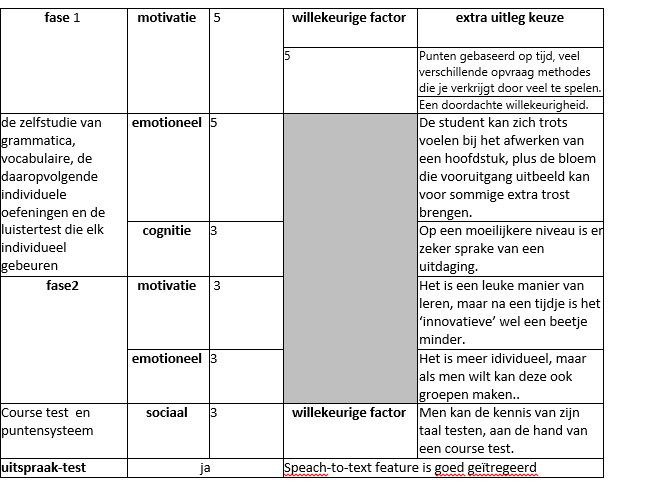
\includegraphics[width=0.7\linewidth]{img/screenshot001}
    \caption{}
    \label{fig:screenshot001}
\end{figure}

% TODO: \usepackage{graphicx} required
\begin{figure}
    \centering
    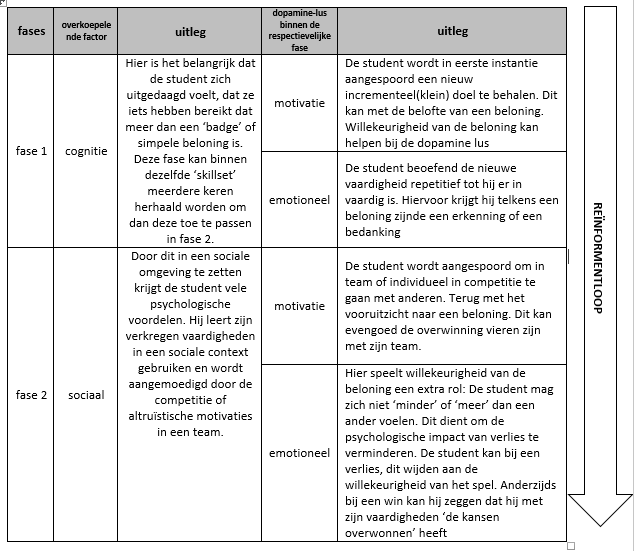
\includegraphics[width=0.7\linewidth]{img/screenshot005}
    \caption{}
    \label{fig:screenshot005}
\end{figure}

Aan de hand van dit schema gaan we in het volgende hoofdstuk verscheidene game-elementen beoordelen.
Welke game elementen sporen aan tot de meest doeltreffende leerervaring.
Inleiding
In dit hoofdstuk beoordelen we de eerste [4] tools die online te vinden zijn om een taal te leren. Hier proberen we op elkaar lijkende tools te vermijden zodat we een beeld krijgen van het bestaande spectrum. Daarna bekijken we een aantal strategieën uit het secondair onderwijs en een paar tools in VR. We beoordelen elk van deze strategieën met een score van 0 tot 5 op ieder vooropgestelde leerfactoren. Bij deze opsomming houden we rekening met nog een onvermelde factor: uitspraak. Deze wordt vaak weggelaten in de gamificatie literatuur omdat die niet gemakkelijk te testen is we zoeken op google: ‘taal leren’ 

% TODO: \usepackage{graphicx} required
\begin{figure}
    \centering
    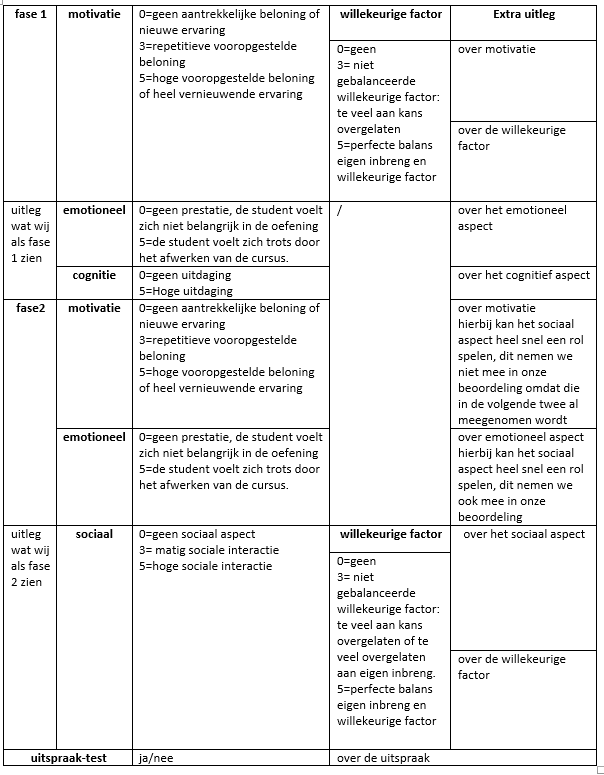
\includegraphics[width=0.7\linewidth]{img/screenshot006}
    \caption{}
    \label{fig:screenshot006}
\end{figure}


Opsomming

NHA[13]
we beginnen met NHA, we doorlopen een proefles. Hierbij hebben we een boek nodig, deze hebben we online een pdf voor gevonden. In het boek staan eerst pagina’s grammatica en vocabulaire die hierna getest wordt. op het einde is er een verbeter sleutel. Er zijn 2 luister opdrachten en 3 leer oefeningen. Dit is duidelijk voor klassikaal gebruikt bedoeld. Hier zijn weinig ludieke elementen en is duidelijk niet gemaakt met deze aspecten niet in gedachten. Dit dien als ‘eiking’ beoordeling

% TODO: \usepackage{graphicx} required
\begin{figure}
    \centering
    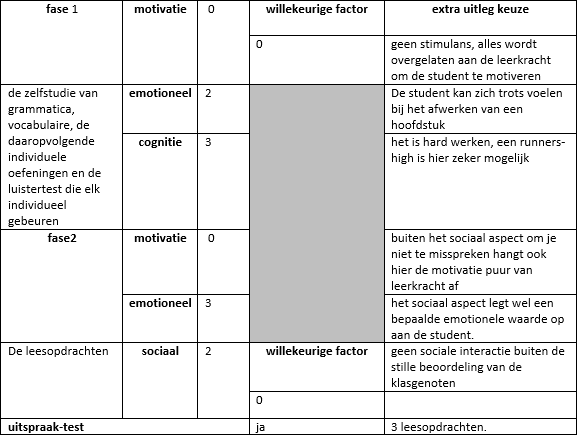
\includegraphics[width=0.7\linewidth]{img/screenshot007}
    \caption{}
    \label{fig:screenshot007}
\end{figure}

Duolingo[14]
We hebben op youtube een walkthrough van een test bekeken, een tutorial en een aantal reviews, extra informatie(leaderbords) direct opgezocht en een aantal mensen die deze app gebruiken aangesproken. Duolingo gaat als volgt te werk: iedere dag krijg je de mogelijkheid om een opdrachtreek uit te voeren, hiervoor heb je 5 levens, bij 5 foutieve antwoorden verlies je en mag je niet meer verder spelen. Deze opdrachten worden semi-willekeurig gekozen en variëren van juiste vervoegingen selecteren tot  zinnen inspreken die dan met speach-to-text technologie beoordeeld worden. Door deze opdrachten te volbrengen krijg je punten die je op een leaderbord plaatst, als je  lang geen opdrachten vervuld verlies je punten. Hiernaast heb je een storymode waarmee je gesprekken aangaat met realistische personages. je moet in die gesprekken woorden en zinnen kiezen die toepasselijk zijn op de geschetste situatie.

% TODO: \usepackage{graphicx} required
\begin{figure}
    \centering
    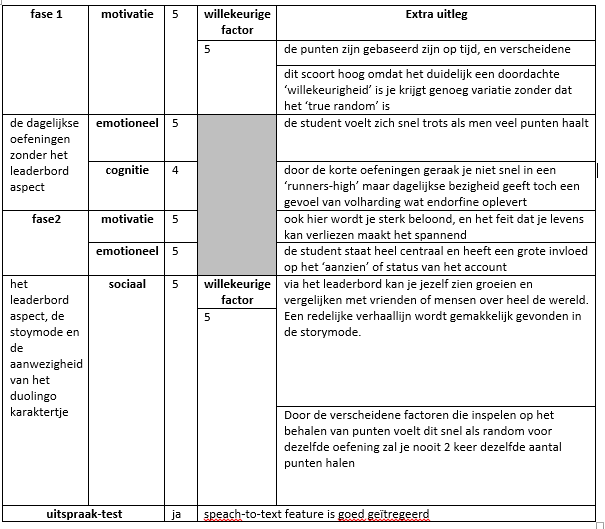
\includegraphics[width=0.7\linewidth]{img/screenshot008}
    \caption{}
    \label{fig:screenshot008}
\end{figure}

loecsen[15]
Loecsen is een gratis website waar je snel basis conversaties, voor als je op vakantie bent, kan leren. Je begint met de belangrijkste uitdrukkingen maar je kan altijd van hoofdstuk veranderen. Er is een vooruitgang-bar voorzien voor iedere hoofdstuk. per hoofdstuk begin je met het aflopen van de vocabulaire. Dit kan je op 2 manieren doen, er is een lijst met gewoon alle woorden en de vertaling. anders is er een lijst met alleen de (in mijn geval)Nederlandse woorden, je kan klikken op ieder woord en er komt een tekening van het woord met de vertaling erboven en iemand die het uitspreekt, bij ieder woord kan je klikken op een microfoon, hij herhaald de uitspraak en vraagt dan aan jou om het woord te herhalen. als je alles hebt ingeoefend kan je op “start een quiz” klikken, die je dan opvraagt per 7 random gekozen woorden, ook hier kan je kiezen om de microfoon functie te gebruiken om je uitspraak te testen.

% TODO: \usepackage{graphicx} required
\begin{figure}
    \centering
    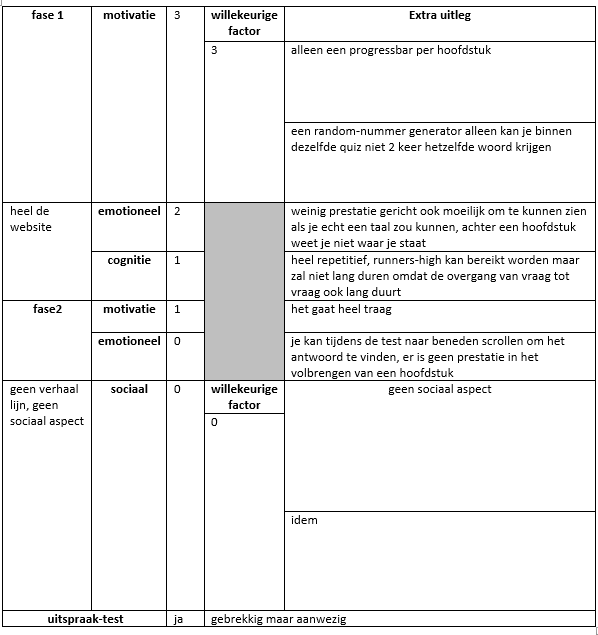
\includegraphics[width=0.7\linewidth]{img/screenshot009}
    \caption{}
    \label{fig:screenshot009}
\end{figure}

Memrise[16]
Memrise is werd in 2017 bekroont tot ‘best app’ in de google play awards. Op de site starten we met aan te duiden welke taal men spreekt en wil leren. Achter dat men beide gekozen heeft, kun je kiezen voor het moeilijkheidsniveau. De cursus gaat van start, je ziet een video met een persoon die een woord uitspreekt en vaak ook een beweging,... maakt. Men vindt ook nog andere zaken terug zoals het uitgesproken woord zelf als ook de Nederlandse vertaling. Er zijn ook andere unieke zaken die we terug kunnen vinden namelijk twee knoppen om de audio opnieuw af te spelen, één met een vrouwen stem en een andere met een mannen stem. Verder ziet men nog een bloem die weergeeft hoe ver je staat met het opnemen van het woord. Het laatste wat men nog kan doen is het woord markeren als moeilijk of weghalen uit zijn woorden lijst.  

% TODO: \usepackage{graphicx} required
\begin{figure}
    \centering
    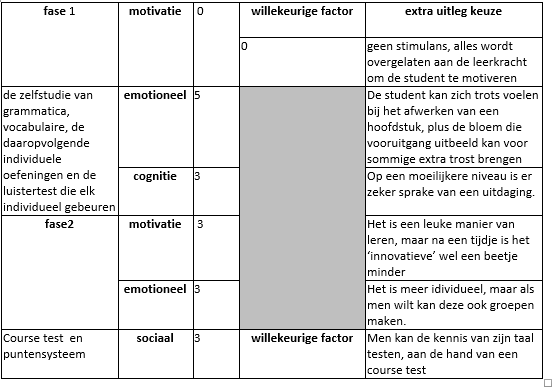
\includegraphics[width=0.7\linewidth]{img/screenshot010}
    \caption{}
    \label{fig:screenshot010}
\end{figure}

Gymlish[17]
Gymlish een verhaallijn gedreven taalcursus, je krijgt teksten, filmpjes of audiofragmenten die bijna allemaal te maken hebben met het ‘Delavigne’ bedrijf. Dit bedrijf is verzonnen door gymlish en volgt je heel de cursus lang. Ze vragen aan jou wat je niet verstaat in de teksten en om inhoudelijke vragen over de tekst de beantwoorden. Ook smijten ze om de zoveel tijd een aantal gramaticale vraagstukken er tussen om te testen als je zelf de gramatica kunt toepassen in andere contexten. achter iedere les krijg je een stukje cultuur of feiten mee om je culturele kennis bij te schaven.

% TODO: \usepackage{graphicx} required
\begin{figure}
    \centering
    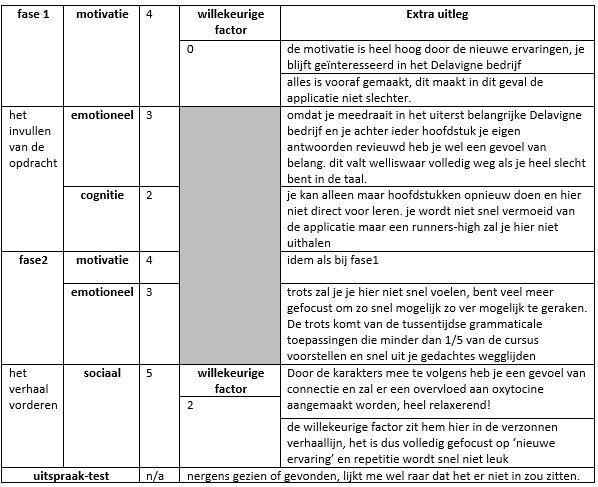
\includegraphics[width=0.7\linewidth]{img/screenshot011}
    \caption{}
    \label{fig:screenshot011}
\end{figure}


\section{Methodologie}

% TODO: (fase 5) beschrijf in detail in welke fasen je onderzoek uiteenvalt, hoe lang elke fase duurt en wat het concrete resultaat van elke fase is. Welke onderzoekstechniek ga je toepassen om elk van je onderzoeksvragen te beantwoorden? Gebruik je hiervoor experimenten, vragenlijsten, simulaties? Je beschrijft ook al welke tools je denkt hiervoor te gebruiken of te ontwikkelen.

Om relevante literatuur te bekomen werd er gezocht op Google Scholar en databases zoals EBSCO en INVERT.

\section{Verwachte conclusies}

% TODO: (fase 6) beschrijf wat je verwacht uit je onderzoek en waarom (bv. volgens je literatuuronderzoek is softwarepakket A het meest gebruikte en denk je dat het voor deze casus ook het meest geschikt zal zijn). Natuurlijk kan je niet in de toekomst kijken en mag je geen alternatieve mogelijkheden uitsluiten. In de praktijk gebeurt het ook vaak dat een onderzoek tot verrassende resultaten leidt, dat maakt het proces nog interessanter!

Niet alleen het dopaminehormoon heeft invloed op het leren, ook andere hormonen spelen hier een rol in. Hoewel blijkt dat er nog veel onderzoeksvragen niet beantwoord zijn, wordt de reinforcingloop gebruikt om de verhouding tussen dopamine en leren te verklaren:
Inspanning blijft de grootste factor bij het aanleveren van nieuwe vaardigheden, zowel bij taal als andere zaken. Dopamine heeft een grote invloed op het maken van beslissingen m.b.t inspanningen. hierbij komen wel een complex aantal externe factoren bij kijken zoals vermoeidheid, belang van de inspanning, perceptie van de grootte van de beloning,.. en ook de perceptie van wat inspanningen inhouden kan een effect hierop hebben. Hierover wordt veel gedebatteerd in de academische wereld. Welke soorten dopaminereceptoren voor welke gedragingen instaan kunnen moeilijk onderzocht worden door gebrek aan duidelijke oriëntatiepunten in het brein. Wat we wel kunnen vaststellen is dat onverwachte beloningen dopamine stimuleren.


%------------------------------------------------------------------------------
% Referentielijst
%------------------------------------------------------------------------------
% TODO: (fase 4) de gerefereerde werken moeten in BibTeX-bestand
% bibliografie.bib voorkomen. Gebruik JabRef om je bibliografie bij te
% houden.

\phantomsection
\printbibliography[heading=bibintoc]



\end{document}
